\documentclass{ntuthesis}

\usepackage{times}
\usepackage{verbatim}
\usepackage{color}
\usepackage{url}
\usepackage{graphicx}
\usepackage{array}

\usepackage{titlesec}
\usepackage{titletoc}

% Centering the ToC's title
\usepackage{tocloft}

% Include ToC/LoF/LoT into ToC
\usepackage[notbib]{tocbibind}

% Include outside .pdf
\usepackage{pdfpages}

% Add wallpaper
\usepackage{wallpaper}

% 2 words indent in first line for Chinese
\usepackage{indentfirst}
\setlength{\parindent}{2em}

% Using the tex-text mapping for ligatures etc.
\defaultfontfeatures{Mapping=tex-text}

% Set the default fonts
\setmainfont{Times New Roman}
%\setCJKmainfont{楷體-繁}
\setCJKmainfont{標楷體}
% value > 0
\def\xeCJKembold{0.4}

% hack into xeCJK, you don't need to understand it
\def\saveCJKnode{\dimen255\lastkern}
\def\restoreCJKnode{\kern-\dimen255\kern\dimen255}

% save old definition of \CJKsymbol and \CJKpunctsymbol for CJK output
\let\CJKoldsymbol\CJKsymbol
\let\CJKoldpunctsymbol\CJKpunctsymbol

% apply pdf literal fake bold
\def\CJKfakeboldsymbol#1{%
  \special{pdf:literal direct 2 Tr \xeCJKembold\space w}%
  \CJKoldsymbol{#1}%
  \saveCJKnode
  \special{pdf:literal direct 0 Tr}%
  \restoreCJKnode}
\def\CJKfakeboldpunctsymbol#1{%
  \special{pdf:literal direct 2 Tr \xeCJKembold\space w}%
  \CJKoldpunctsymbol{#1}%
  \saveCJKnode
  \special{pdf:literal direct 0 Tr}%
  \restoreCJKnode}
\newcommand\CJKfakebold[1]{%
  \let\CJKsymbol\CJKfakeboldsymbol
  \let\CJKpunctsymbol\CJKfakeboldpunctsymbol
  #1%
  \let\CJKsymbol\CJKoldsymbol
  \let\CJKpunctsymbol\CJKoldpunctsymbol}
\newcommand\zhbf[1]{\CJKfakebold{#1}}

% Very Naive Chinese Number
\newcommand\naiveZhNum[1]{
\ifnum #1 = 1 
一 
\else \ifnum #1 = 2
二
\else \ifnum #1 = 3
三
\else \ifnum #1 = 4
四
\else \ifnum #1 = 5
五
\else \ifnum #1 = 6
六
\else \ifnum #1 = 7
七
\else \ifnum #1 = 8
八
\else \ifnum #1 = 9
九
\else
#1
\fi\fi\fi\fi\fi\fi\fi\fi\fi
}


% ToC, LoF, LoT centering settings with package tocloft
\renewcommand{\cftloftitlefont}{\hfill \Huge}
\renewcommand{\cftafterloftitle}{\hfill}
\renewcommand{\cfttoctitlefont}{\hfil \Huge}
\renewcommand{\cftaftertoctitle}{\hfill}
\renewcommand{\cftlottitlefont}{\hfill \Huge}
\renewcommand{\cftafterlottitle}{\hfill}

\titleformat{\chapter}{\centering\Huge\bfseries}{第\,\naiveZhNum{\thechapter} \,章}{1em}{}
\renewcommand{\cftchapleader}{\cftdotfill{\cftdotsep}} % dots for chapters
\titlecontents{chapter}[0em]{}{\makebox[4.1em][l]{第\naiveZhNum{\thecontentslabel}章}}{}{\cftdotfill{\cftdotsep}\contentspage}

% Your information goes here
% author: Tz-Huan Huang [http://www.csie.ntu.edu.tw/~tzhuan]

% ----------------------------------------------------------------------------
% "THE CHOCOLATE-WARE LICENSE":
% Tz-Huan Huang wrote this file. As long as you retain this notice you
% can do whatever you want with this stuff. If we meet some day, and you think
% this stuff is worth it, you can buy me a chocolate in return Tz-Huan Huang
% ----------------------------------------------------------------------------

% modify by Qing-Cheng Li (qcl) [http://qcl.github.io/]

% Syntax: \var{English}{Chinese}
\university{National Taiwan University}{國立臺灣大學}
\collage{College of Electrical Engineering and Computer Science}{電機資訊學院}
\institute{Department of Computer Science and Information Engineering}{資訊工程學研究所}
\title{TBA}{巨量文件中樣式與屬性關聯性之分析}
\author{Qing-Cheng Li}{李卿澄}
\studentid{R01922024}
\advisor{Hsin-Hsi Chen, Ph.D.}{陳信希 博士}
\year{2014}{103}
\month{July}{7}
\day{31}


% Modify some default titles for Chinese
\renewcommand{\contentsname}{目錄}
\renewcommand{\listfigurename}{圖目錄}
\renewcommand{\listtablename}{表目錄}
\renewcommand{\tablename}{表}
\renewcommand{\figurename}{圖}
\renewcommand{\bibname}{參考文獻}

\begin{document}

% 臺大論文浮水印
%\CenterWallPaper{0.174}{pdfs/watermark.pdf}
%\setlength{\wpXoffset}{6.1725cm}
%\setlength{\wpYoffset}{10.5225cm}

\frontmatter

\makecover
%\makespine % TODO

% 口試委員會審定書 TODO 
% 以 \makecertification 產生
%\makecertification
% 或匯入外部.pdf檔
%\addcontentsline{toc}{chapter}{口試委員會審定書}
%
\includepdf[pages={1}]{pdfs/cert.pdf}

% 誌謝 TODO
%\begin{acknowledgementszh}
感謝\ldots
\end{acknowledgementszh}

\begin{acknowledgementsen}
I'm glad to thank\ldots 
\end{acknowledgementsen}

% 摘要
% 中文摘要
\begin{abstractzh}

世界上的知識日新月異,
透過志願編輯者更新的知識庫無法跟上知識產生與改變的速度,
如何縮短知識產生與知識庫更新間的差距,也就是知識庫加速,便成為了重要的議題。

知識庫中記載的實體與其特性也是相當重要的知識,
本研究提出了基於樣式,
自資訊匯集而成之內容串流中快速地偵測文件是否包含特定實體特性的方法。
偵測流程包含了樣式比對、樣式篩選與特性消歧義等步驟。
透過樣式比對與實體特性與樣式的關聯偵測實體特性,
這其中存在樣式的品質、可信賴度、對映特性的歧義等問題,
本研究於樣式比對前進行樣式篩選,比對後進行特性消歧義以降低上述問題的影響。

實驗結果分析了樣式信心值、可信賴度、特性歧義度對效能造的影響,
以及發現特性消歧義的步驟中,引入實體類型資訊與使用簡單貝氏分類器後,
偵測效能有顯著的提升。

透過實體特性的偵測,有助於自內容串流中篩選對知識庫更新有幫助的文章以供志願編輯者作為更新與維護知識庫的依據。\\

\noindent
關鍵字:知識庫加速、樣式比對

\end{abstractzh}

% 英文摘要
\begin{abstracten}
\end{abstracten}



% TODO FIXME - Chinese Chapter Wording setting
% Table of Content
\clearpage
\tableofcontents
% List of Figures
\clearpage
\listoffigures
% List of Tables
\clearpage
\listoftables

\mainmatter

% Your thesis goes here
%
%   Chapter Introduction
%
%   author: Qing-Cheng Li r01922024 at csie dot ntu dot edu dot tw
%
\chapter{緒論}
\label{c:intro}

近年來,隨著網際網路的快速發展,網際網路中開始出現越來越多彙整人類知識的網站與資源,
如Wikipedia\footnote{http://www.wikipedia.org/},目前已經有超過280種語言,其中光是英語的條目就超過4,500,000條,
是透過來自世界各地的志願編輯者一字一句的貢獻建立而成的。

除了讓世界各地的人們可以在網際網路上共享知識之外,也讓計算機得以利用人類的知識,
輔助、改善、甚至自動化人工智慧、資料探勘與擷取、知識汲取、自動問答系統等任務,

為了達成此一目的,讓計算機可以看懂人類的知識,於是,
便出現了各式各樣透過擷取人工建立的知識資源,產生的結構化知識資料庫,並彼此相互鏈結。
如圖\ref{i:lod}所示,目前已有不少的結構化知識庫。
這些各式各樣的資源的最源頭,還是透過人類一字一句編輯產生的。% FIXME

\begin{figure}
\centering
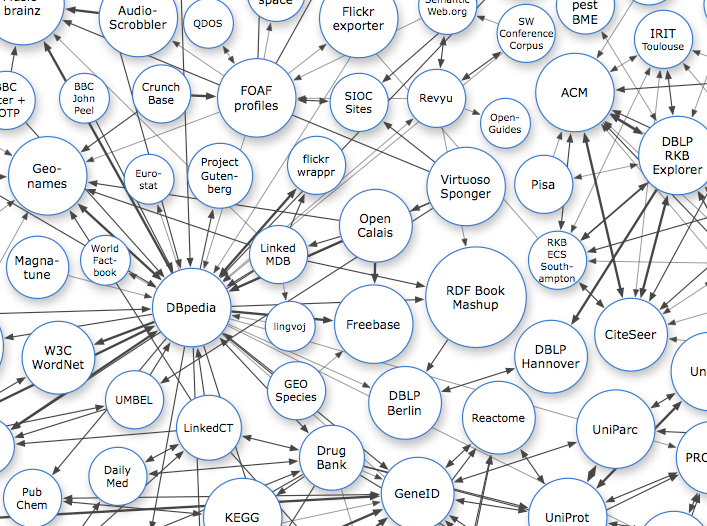
\includegraphics[width=0.5\textwidth]{images/01-lod-datasets}
\caption{各種結構化知識資料庫之間的鏈結}
\label{i:lod}
資料來源:linkeddata.org(2011)
\end{figure}

%
%   Background
%
\section{背景介紹}
在現今這個資訊社會,每當有新的事件發生時,例如某人的出生或死亡、某政治人物贏得了選舉、某地發生了天災等等,
這些資訊便會在網路上透過網路新聞、網誌、論壇、社群網站、微網誌等管道流傳。
新事件的發生代表了一些舊有的知識可能需要更新,例如修改某個人物的生死狀態、某個政治人物的勝選記錄等,
如有Wikipedia的志願編輯者注意到這些資訊之後,便會據此更新Wikipedia上關於某人或某球隊的條目。

如Wikipedia這種用來記錄實體(Entity)、實體的特性(Properties)、實體與實體間的關係(Relationships)的資料庫被稱為知識庫(Knowledge Base)。
以Wikipedia來說,Wikipedia以文章的形式儲存了人物、組織、公司、城市、事件等實體,
並在文章的文句中以超連結(Hyperlink)的形式描述實體與實體間的關係。
而文章中的資訊框(Infoboxes)則以半結構化的形式描述了實體的特性,如圖\ref{i:wiki}。

\begin{figure}
\centering

\includegraphics[width=0.65\textwidth]{images/01-wiki-as-kb}
\caption{Wikipedia中的文章}
\label{i:wiki}
\end{figure}

除了Wikipedia之外,還有其他DBpedia\cite{dbpedia-swj}、YAGO\cite{suchanek2007WWW}、Freebase\cite{freebase}等規模大小不一、不同應用的知識庫。
其中YAGO、DBpedia是透過自動化的方法擷取Wikipedia的內容,Freebase仰賴社群更新,這些知識庫都直接或間接仰賴人力更新。  %FIXME

%
%   Motivation
%
\section{研究動機}
% 知識庫不會憑空產生,多半是擷取人工編輯的成果或靠人工編輯,因此如何讓人工編輯的速度可以跟上知識產生的速度便成為一個重要的課題。
% TODO
% Keyword: 知識庫加速
知識庫仰賴志願編輯者的維護與更新,但這些人數比起資料庫中記錄的實體顯然非常的少。
這意味著知識庫的更新總是落後於新知識(過去從來不知道的知識與舊有知識內容的更動)的產生,
當新知識產生一段時日之後,知識庫的維護者才會更新知識庫,
圖\ref{i:wikicitenews}\cite{kba2012}表現了這種落後可能達一年甚至更長。
因此,如何讓人工編輯的速度可以跟上新知識出現的速度便成為一個重要的課題。

\begin{figure}
    \centering
    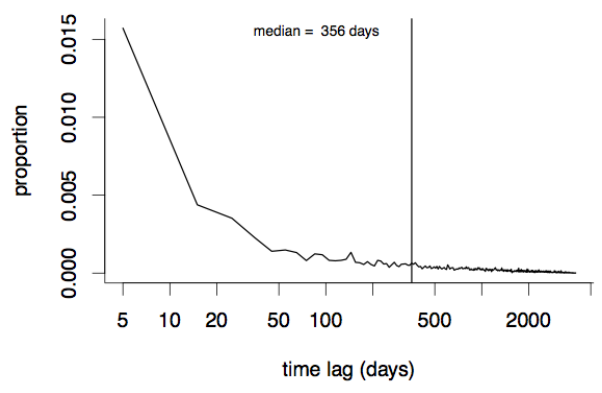
\includegraphics[width=0.5\textwidth]{images/01-wiki-cite-delay}
    \caption{Time lag for a sample of ~60,000 web pages cited by WP articles}
    \label{i:wikicitenews}
\end{figure}

為了縮短這個差距,自2012年起至今的每年美國NIST\footnote{National Institue of Standards and Technology}的TREC\footnote{Text Retriveal Conference}都會舉辦知識庫加速(Knowledge Base Acceleration, KBA)競賽,
希望參賽者可以建立一個系統,從由新聞、部落格、論壇等內容所組成、依時間所排列的龐大內容串流\footnote{2012年包含了4,973個小時,2013年包含了11,948小時。每小時包含約100,000份文件。}(Content Strean)中,
對有興趣的實體\footnote{2012年有27個人物、2個組織,2013年有98個人物,12個組織與24個設施。},包含了人物、組織或建築,進行過濾,
推薦文件給知識庫的編輯者,建議編輯者這份文件可能含有新的知識可供更新知識庫。

要從可能包含新知識的內容串流中,過濾出可能可以協助更新知識庫的文件,
則需要知道文章中是否包含知識。知識庫中實體間的關係、實體的特性就是一種知識,
我們想要知道一份來自內容串流的文件是否提及實體的特性,
例如句子「Jobs was born in San Francisco, California on February 24, 1955」中就包含了實體Jobs及其出生地這項特性的知識。
如果可以知道文章中是否包含這些資訊,便能夠進一步地協助知識庫的更新與維護。

% TODO
% We want to fill the Knowledge gap, do it fast

%
%   Goal
%
\section{研究目標}
% Keyword: given a content stream, 回答有沒有某個特性這樣
% TODO

%
%   Structure
%
\section{論文架構}  % TODO FIXME
本論文共分成五個章節。
第一章是緒論,簡介本研究的背景、動機與目標。
第二章是文獻探討,列舉了一些相關的研究與資源。
第三章是研究方法,提出如何於內容串流中究偵測實體特性的方法與步驟。
第四章是實驗結果與分析,
第五章是結論與未來展望,

   % FIXME
%
%   Chapter Related Works
%
%   Qing-Cheng Li (r01922024 at csie dot ntu dot edu dot tw)
%   R.O.C.103.07
%
\chapter{相關研究與文獻}
\label{c:related}

% FIXME - 需要潤飾。
本章將介紹相關的研究:知識庫加速(Knowledge Base Acceleration)方面相關的研究,
及相關的資源:結構化的知識庫(Structural Knowledge Bases)與實體間的關係(Relations between Entities)。

%
%   KBA
%
\section{知識庫加速}

\cite{kba2012}與\cite{kba2013}整理了2012年、2013年TREC的知識庫加速競賽的總覽。
\cite{kba2012}追蹤60,000個被Wikipedia引用的網頁,
發現引用文章的時間與被引用文章的產生時間差中位數是一年,
顯示知識庫更新的速度遠落後於知識產生的速度,為了彌補這個差距,
連續兩年皆有累積引用推薦(Cumulative Citation Recommendation, CCR)任務,   % FIXME - 翻譯?
有一個特定的實體清單,並從內容串流中篩選出值得被引用的文件來建議知識庫的編輯者更新及維護知識庫。

% 內容串流描述

% 競賽結果簡述

% 圍繞「實體」為主的方法。
\cite{kba-hltoce}利用什麼方法,
而\cite{kba-msra}用的方法是,

% 除此之外...
另外,\cite{kba-entity-detection}

%
%   Structural KB
%
\section{結構化的知識庫}
% TODO

\cite{freebase}
\cite{dbpedia}
\cite{yago}

\cite{freebase-qa-extract}
\cite{freebase-qa-parse}
\cite{yago-qa}

\cite{aptagger}
%
%   Pattern and Relation
%
\section{實體間的關係}

知識隨著時間變化是可能產生改變的,
\cite{relationsByTime} 提到有些實體間的關係是相對恆常的,例如《1Q84》的作者是村上春樹;
而有些關係則是隨著時間而變動的,例如美國的總統是布希,只有在某一段時間內是正確關係。
此研究將實體間的關係分為是否為恆常(Constant)或是否唯一(Unique),
人工挑選1,000組關係並利用時間、實體出現在特定時段內的頻率、文法等特徵對關係進行分類。

\cite{reverb} 建立了一套開放資訊擷取系統(Open Information Extraction System),
透過動詞表示的詞彙與句法限制,以<arg1, relation, arg2>的形式自動擷取出實體間的關係,
不限於人工標定的關係。

而Wikipedia中,每一篇文章,或稱條目,是描寫一個特定的實體,
\cite{wisenet} 利用Wikipedia文章中連至其他條目的連結作為實體,
以此擷取條目間,也就是實體間的關係。
由於同一種關係可能由不同的語句樣式(Patterns)來表達,
此研究應用了Wikipedia條目分類資訊、樣式的前後文來分類同義樣式。

\cite{patty2012}及\cite{patty}建立了一個名為PATTY的分類集(Taxonomy),
將用來表達關係的樣式進行分類,將同義樣式合併,並附上實體類別資訊,
將關係表達為「<type 1> \emph{Pattern} <type 2>」,Type 1和Type 2是實體的類別,
而Pattern則由單字(Words)、詞性標記(Part-Of-Speech Tags)、萬用字元(Wildcards)所組成,
例如「<person>'s [adj] voice * <song>」。   % FIXME - Example

PATTY自Wikipedia、New York Times抽取句子,
以史丹佛剖析器(Stanford Parser\footnote{http://nlp.stanford.edu/software/lex-parser.shtml})對句子建立剖析樹,
以YAGO、Freebase作為實體的字典,判斷若句子中有兩個實體,
則把兩實體間在樹上的最短路徑上的字句擷取出來作為樣式,
並進一步合併樣式為同義樣式集(Pattern Synset)。
比起\cite{reverb},PATTY可以抽取任意的關係,不被詞彙或句法所限制。

對每一個樣式,都存在一組支持集(Support Set),
由符合樣式的實體對(Pairs of entites)所組成。
透過支持集的大小,對每個樣式計算計算了一個信心值(Confidence),
將樣式中的實體類別從類別改為類別繼承架構中的更廣義的父節點類別,
以可以填入的實體對數作為分母,支持集作為分子,
得到的分數就是心信值,代表一個樣式的品質。

除了同義樣式集之外,此研究還做了關係釋義(Relation Paraphrasing):
給定一個來自知識庫的關係,判斷一個樣式是否可以描述此一關係。
PATTY釋義了225種DBpedia關係,包含127,811個樣式;25種YAGO關係,包含43,124個樣式。
其透過隨機選取1,000組釋義來評估,平均的精確度(Precision)是0.76$\pm$0.03。

本研究將嘗試利用PATTY提供的關係釋義來偵測實體特性是否存在於文件之中。   % FIXME - 收尾好像不是收的挺好

        % TODO
%%
%   Chapter Method
%
%   Qing-Cheng Li (r01922024 at csie dot ntu dot edu dot tw)
%   R.O.C.103.07
%
\chapter{方法}
\label{c:method}

\section{樣式比對}

\section{樣式挑選}


        % TODO 
%\input{chapters/experiments}   % TODO
%%
%   Chapter Conclusion
%
%   Qing-Cheng Li (r01922024 at csie dot ntu dot edu dot tw)
%   R.O.C.103.07
%
\chapter{結論與未來展望}
\label{c:future}

\section{結論}
有別於過去的研究多半著重於於內容串流中找尋實體相關的文件,
本研究專注於於內容串流中尋找實體的特性,
提出了於基於樣式於內容串流中偵測實體特性的方式。
自內容串流中比對樣式,透過實體特性與樣式間的關聯,
快速地偵測文件是否包含特定的實體樣式。
由於偵測流程文件與文件是互相獨立的,
整個偵測的流程可平行化,具備可擴展性,
能夠處理模擬真實世界的內容串流。

本研究也為偵測特性的過程加入了樣式篩選與特性消歧義等步驟以提升偵測效能。
樣式篩選針對了樣式信心值、可信賴程度以及樣式歧義度三個面向進行篩選。
對樣式篩選越嚴格,則可以使用的樣式越少,因此召回率會下降。
例如對信心值進行篩選,精確率有提升,但整體效能仍下降;
對可信賴度進行篩選,精確率隨有提升但隨著門檻提高,太高的門檻反而使整體效能下滑。
而採用歧義度越高的樣式,則可採用的樣式總數增加,召回率有提升,而整體效能緩步下滑。

特性消歧義的步驟則是進行於樣式比對之後,
用以區辨樣式出現的地方是否無實體特性或有實體特性,是一個或多個實體特性。
透過引入實體類型資訊捨去不符合條件的特性,可在不改變召回率的情形下使系統的效能有顯著的提升。
針對特性的篩選實驗了四種篩選策略,由宏觀平均的角度來看,選擇正規化後正確率大於0.5的特性是最有幫助的。
最後再透過簡單貝氏分類器對特性進行存在或不存在的二元分類,可以顯著提升系統效能。
總體而論,結合引入實體類型資訊、選擇正規化後正確率大於0.5的特性後以簡單貝氏分類器進行分類可以得到最好的系統效能。

\section{未來展望}
就偵測流程本身,分析錯誤主要來自,第一類是來自歧義性,
第二類是無法分辨有無特性存在,以及第三類覆蓋度不足。
其中以第二類為影響精確率的主要錯誤來源,
如何消彌這幾種錯誤以繼續改善偵測效能是未來的研究課題之一。

而本研究所使用之樣式,以及樣式與實體特性之關聯表來自於PATTY,
在樣式的覆蓋度以及與實體特性間的關聯度強弱受到一定程度的限制,
在未來希望可以自網路資源擷取樣式降低覆蓋度的影響,
並與知識庫特性建立更細緻的關聯,以降低歧義性造成的影響。

關於測試資料集,因為沒有正確的答案標記,只能透過YAGO來進行推測,
並假設所有的語句都是描寫該條目,希望未來可以針對文件,
甚至到句子等級的答案標記,可以進行更詳細的研究。
本研究目前是針對文件等級進行偵測,若有更細緻的答案標記,
或許可以進行句子等級的偵測。
更進一步,希望能夠知道句子中樣式描述的對象實體與其在句子中的位置,
才能更精確地偵測實體特性。
而Wikipedia的條目屬於較長的文章,也希望未來可以針對微網誌、社群留言等短訊息進行偵測。
使得偵測的面向更為廣泛以及更為細緻,甚至是自動化地對知識庫進行更新。

    % TODO

\appendix

\backmatter

\addcontentsline{toc}{chapter}{\bibname}
\bibliographystyle{ieeetr}  % use ieeetr, so the order will sort by apperance

% Your bibliography goes here
\bibliography{thesis}

\end{document}
